
\documentclass[twocolumn]{article} % default is 10 pt
\usepackage{graphicx} % needed for including graphics e.g. EPS, PS

\long\def\comment#1{}

% uncomment if don't want page numbers
\pagestyle{empty}

%set dimensions of columns, gap between columns, and paragraph indent

\setlength{\textheight}{9.5in} \setlength{\columnsep}{1pc}
\setlength{\textwidth}{7in}

\setlength{\topmargin}{0in}

\setlength{\headheight}{0.0in}
\setlength{\headsep}{0.0in}
\setlength{\oddsidemargin}{-0.35in}
\setlength{\evensidemargin}{-0.35in}
\setlength{\parindent}{0pt}
\setlength{\parskip}{0.12in}
\makeatletter
\def\@normalsize{\@setsize\normalsize{10pt}\xpt\@xpt
\abovedisplayskip 10pt plus2pt minus5pt\belowdisplayskip
\abovedisplayskip \abovedisplayshortskip \z@
plus3pt\belowdisplayshortskip 6pt plus3pt
minus3pt\let\@listi\@listI}

%need an 11 pt font size for subsection and abstract headings
\def\subsize{\@setsize\subsize{12pt}\xipt\@xipt}
%make section titles bold and 12 point, 2 blank lines before, 1 after
\def\section{\@startsection {section}{1}{\z@}{1.0ex plus
1ex minus .2ex}{.2ex plus .2ex}{\large\bf}}
%make subsection titles bold and 11 point, 1 blank line before, 1 after
\def\subsection{\@startsection
   {subsection}{2}{\z@}{.2ex plus 1ex} {.2ex plus .2ex}{\subsize\bf}}
\makeatother


% GENERAL MACROS
\newcommand{\bc}{\begin{center}}
\newcommand{\ec}{\end{center}}
\newcommand{\beq}{\begin{equation}}
\newcommand{\eeq}{\end{equation}}
\newcommand{\bea}{\begin{eqnarray}}
\newcommand{\eea}{\end{eqnarray}}
\newcommand{\ba}{\begin{array}}
\newcommand{\ea}{\end{array}}

\def\ie{{\it i.e. }}
\def\eg{{\it e.g. }}
\def\etal{{\it et. al. }}

% PDE MACROS
\def\tu{\tilde{u}}
\def\abar{\bar{a}}
\def\cbar{\bar{c}}
\def\dbar{\bar{d}}

% NUMERICS MACROS
\def\dt{\Delta t}
\def\dx{\Delta x}
\def\dy{\Delta y}
\def\pt{\partial t}
\def\px{\partial x}
\def\dto{\Delta t_{opt}}
\def\he{\hat{e}}


\begin{document}
\bibliographystyle{unsrt}

% don't want date printed
\date{}

% >>>>>>>>>>>>>>>>>>>>>>>  Put your title here <<<<<<<<<<<<<<<<<<<<<<<<
% make title bold and 14 pt font (Latex default is non-bold, 16pt)
\title{\huge \bf {Using Optimal Time Step Selection to \\ 
       Boost the Accuracy of FD Schemes for \\
       Variable Coefficient PDEs }}

% >>>>>>>>>>>>>>>>>>>>>>> Author's Name, Thanks or Affliation <<<<<<<<
\author{Kevin T. Chu\thanks{
  K.T. Chu gratefully acknowledges the support of Vitamin D, Inc.
  and the Institute for High-Performance Computing (IHPC) in Singapore. 
  Vitamin D, Inc., Menlo Park, CA 94025 \& 
  Institute of High Performance Computing, A*STAR, Singapore, Singapore.
  Email: ktchu@serendipityresearch.org.
  Manuscript submitted 2009 March 20. 
 } 
 \ and
 James V. Lambers\thanks{Department of Energy Resources Engineering, 
 Stanford University, Stanford, CA 94305.  Email: lambers@stanford.edu.}
}

\maketitle
\thispagestyle{empty}

% >>>>>>>>>>>>>>>>>>>>>>>>> Keywords and Abstract <<<<<<<<<<<<<<<<<<<<<
{\hspace{1pc} {\it{\small Abstract}}{\bf{\small---We extend the technique 
of optimal time step (OTS) selection for finite difference (FD) schemes of time 
dependent PDEs to PDEs where the leading-order spatial derivative term has a
spatially varying coefficient.  The basic approach involves identifying a 
transformation of the domain that eliminates the spatial dependence of the 
coefficient for the leading-order term.  This change of variables is then used 
to define an optimal computational grid for the FD scheme on the 
\emph{original} domain.   By using both the optimal grid and OTS selection, we are
able to boost the order of accuracy above what would be expected from a formal
analysis of the FD scheme.  We illustrate the utility of our method by 
applying it to variable coefficient wave and diffusion equations.  In 
addition, we demonstrate the viability of OTS selection for the two-step 
Kreiss-Petersson-Ystr\"om discretization of the wave equation.

\em Keywords: optimal time step selection, optimal grid selection, finite 
    difference schemes, time dependent PDEs, variable coefficient PDEs}}
 }

% >>>>>>>>>>>>>>>>>>>>>> START OF PAPER <<<<<<<<<<<<<<<<<<<<<<<<<<<<<<
\section{Introduction}
\label{Introduction}
Optimal time step (OTS) selection is a surprisingly simple and effective way to 
boost the order of accuracy of finite-difference (FD) schemes for 
time-dependent partial differential equations~\cite{chu_otspde}.  The basic
principle underlying OTS selection is that a careful choice of time step (and 
the addition of a few correction terms) can boost the \emph{order} of 
accuracy for formally low-order finite difference schemes.  For instance, it 
is possible to obtain a fourth-order accurate solution of the 1D diffusion 
equation using only the standard second-order central difference approximation 
and forward Euler time integration.  As demonstrated in~\cite{chu_otspde}, OTS 
selection works for linear and semilinear PDEs in any number of space 
dimensions on both regular and irregular domains.  

Unfortunately, a limitation of the existing formulation of OTS selection is 
the requirement that the leading-order spatial derivative of the PDE have a 
constant coefficient.  In this paper, we remove this limitation and extend OTS 
selection to general variable-coefficient semilinear PDEs.  
Our approach is to identify a transformation of the domain which 
eliminates the spatial dependence of the coefficient on the leading-order 
spatial derivative.  Using this transformation, we define an optimal 
computational grid which can be used in conjunction with OTS selection to 
boost the order of accuracy of formally low-order FD schemes for the PDE.  
Optimal grid selection is an important extension of the philosophy that the 
accuracy of numerical methods can be boosted via optimization of the 
parameters used to compute the solution.

This paper is organized as follows.  First, we briefly review OTS selection 
for PDEs with a constant-coefficient leading-order spatial derivative term.  
Next, we show how to combine optimal grid and optimal time step selection to 
boost the accuracy of finite difference schemes for variable-coefficient PDEs.  
We then demonstrate the use of variable-coefficient OTS selection on the 
variable-coefficient wave and heat equations.  Our analysis of the wave is 
equation is particularly noteworthy because it is \emph{not} based on a one-step 
time integration scheme.  We conclude with a summary of our main results
and thoughts on future directions for research.


\section{Review of OTS Selection for Constant Coefficient PDEs
  \label{sec:ots_const_coef_pdes}}
Optimal time step selection is not by itself a method for constructing 
finite-difference schemes.  Rather, it is a technique for enhancing the 
performance of existing FD schemes by carefully choosing the time step to 
eliminate low-order numerical errors.  There are two fundamental ideas 
underlying OTS selection.  First, a judicious choice of time step can be 
used to eliminate the leading-order terms in the error.  Second, the PDE 
provides valuable insight into the discretization errors for FD schemes.  
Combining these two simple ideas often yields an optimal time step which 
can be used to \emph{boost} the order of accuracy of a given FD scheme 
above what would be expected from a formal analysis of the scheme.

To illustrate the basic theory behind OTS selection, let us consider the 
constant-coefficient diffusion equation
\beq
  u_{t} = D u_{xx} + f(x,t),
 \label{eq:diffusion_eqn_1d}
\eeq
where $D$ is the diffusion constant and $f(x,t)$ is a source term.  Perhaps
the simplest FD scheme for this equation uses forward Euler time integration 
and the standard second-order central difference approximation for the 
Laplacian:
\beq
  u^{n+1}_j = u^{n}_j
    + \dt
      \left( D \left[\frac{u^{n}_{j+1} -2 u^{n}_j + u^{n}_{j-1}}{\dx^2}\right]
           + f^n_j \right).
 \label{eq:diffusion_eqn_1d_FD_scheme}
\eeq
This scheme is formally first-order in time and second-order in 
space.  The stability constraint $\dt \le \dx^2/2D$ implies that the scheme is
$O(\dx^2)$ accurate overall.  

OTS selection is based on a detailed analysis of the leading-order errors in 
FD schemes.  We begin by deriving the truncation error for the scheme 
(\ref{eq:diffusion_eqn_1d_FD_scheme}).  Employing Taylor series expansions and 
the PDE (\ref{eq:diffusion_eqn_1d}), we find that the true solution satisfies
\bea
  \tu^{n+1}_j &=& \tu^{n}_j
  + \dt \left( D \tu_{xx} + f \right)
  \nonumber \\
  &+& \frac{\dt^2}{2} \left( D^2 \tu_{xxxx} + D f_{xx} + f_t \right)
  + O \left( \dt^3 \right) \ \ 
  \label{eq:diffusion_eqn_1d_time_err}
\eea
and that the central difference approximation for the Laplacian satisfies
\beq
  \frac{\tu^{n}_{j+1} -2 \tu^{n}_j + \tu^{n}_{j-1}}{\dx^2}  =
  \tu_{xx} + \frac{\dx^2}{12} \tu_{xxxx}
  + O(\dx^4).
  \label{eq:diffusion_eqn_1d_space_err}
\eeq
Therefore, the truncation error for (\ref{eq:diffusion_eqn_1d_FD_scheme})
is given by
\bea
  & & \tu_{xxxx}
  \left[ \frac{\dx^2}{12} - \frac{D \dt}{2} \right] (D \dt)
  - \frac{\dt^2}{2} \left( D f_{xx}
  + f_t \right)
  \nonumber \\
  & & + \ O(\dt \dx^4) + O(\dt^3).
  \label{eq:diffusion_eqn_1d_trunc_err}
\eea
From this expression, we see that choosing the time step to be
$\dt = \dx^2/6D$ and adding the correction term 
\beq
  \frac{\dt^2}{2} \left( D f_{xx} + f_t \right)
\eeq
eliminates the leading-order truncation error.  Using the heuristic
argument that the global error is equal to the local error divided by 
$\dt$~~\cite{gko_book}, we find that the numerical solution is 
$O(\dx^4) + O(\dt^2) = O(\dx^4)$ accurate -- the FD scheme has been
boosted from second- to fourth-order accuracy.

As shown in~\cite{chu_otspde}, this general procedure can be used to boost 
the accuracy of FD schemes for any semilinear PDE that has a constant 
coefficient leading-order spatial derivative.  It is important to emphasize 
that variable coefficients and nonlinearities in the lower-order spatial 
derivative terms do not pose a problem for OTS selection.  


\section{OTS Selection for Variable Coefficient PDEs
  \label{sec:ots_var_coef_pdes}}
Transformation of the spatial domain is a natural way to extend OTS selection 
to semilinear PDEs that have variable coefficient leading-order spatial 
derivatives.  Consider a semilinear PDE of the form:
\bea
  \frac{\partial u}{\partial t} = a^n(x) \frac{\partial^n u}{\partial x^n}
 + F \left( \frac{\partial^{n-1} u}{\partial x^{n-1}}, \ldots,
           \frac{\partial u}{\partial x}, u \right)
 + f(x,t)
\label{eq:semilinear_PDE}
\eea
on the domain $0 < x < 1$.  Using the change of variables\footnote{This
transformation is a generalization of the change of variables proposed
in~\cite{guidotti2006} for the wave equation.}
\beq
  y = \Phi(x) = \abar \int_0^x \frac{1}{a(\xi)} d\xi
  \label{eq:change_of_variables}
\eeq
with 
\beq
  \abar \equiv \left( \int_0^1 \frac{1}{a(\xi)} d\xi \right)^{-1},
  \label{eq:abar}
\eeq
we can completely eliminate the spatial dependence of the coefficient on the 
leading-order spatial derivative (at the expense of adding 
lower-order variable-coefficient spatial derivative terms).  The PDE 
(\ref{eq:semilinear_PDE}) on the transformed domain has the form
\bea
  \frac{\partial u}{\partial t} = {\abar}^n \frac{\partial^n u}{\partial y^n}
 + \tilde{F} \left( \frac{\partial^{n-1} u}{\partial y^{n-1}},
           \ldots,
           \frac{\partial u}{\partial y}, u \right)
 + f(y,t),
\label{eq:semilinear_PDE_transformed}
\eea
where $\tilde{F}$ includes any lower-order terms introduced by the process of 
changing variables.

The change of variables (\ref{eq:change_of_variables}) allows us to apply 
OTS selection in one of two ways.  First, we could simply apply OTS selection
to the transformed PDE on the transformed domain.  An important alternative,
however, is to solve the PDE on the \emph{original} domain using a variable 
spaced grid generated by mapping a uniform grid from the transformed to the 
original domain.  Amazingly, OTS selection can be used to boost the accuracy 
of natural choices of finite difference schemes defined on this 
\emph{optimal computational grid}. 

Mathematically, these two approaches are equivalent.  The former approach is 
numerically simpler but requires the solution of a more complicated PDE.
The latter approach places more complexity on the construction of the FD
scheme but requires no modification to the PDE.  When using OTS selection,
the latter approach is generally superior because it dramatically simplifies 
the derivation of the correction terms.


\subsection{Construction of FD Schemes for Optimal Grid}
When constructing FD schemes for the optimal grid on the original domain, it 
is important to define them as divided differences that use grid points 
corresponding to the ones used on the transformed domain.  Doing so ensures 
that the FD scheme for the PDE on the original domain is compatible with the 
FD scheme for the transformed PDE on the transformed domain (\ie the FD scheme 
on the variable spaced grid automatically encapsulates the required 
transformation of the PDE that result from the change of variables).  This 
compatibility preserves the fortuitous cancellation of errors on the optimal 
grid even though it is not uniform.  

For instance, the generalization of the second-order central difference 
operator for the 1D Laplacian on a variable spaced grid is
\bea
  (u_{xx})_i &\approx&
    \frac{1}{(x_{i+1}+x_i)/2 - (x_i+x_{i-1})/2}
  \nonumber \\
    & & \times \left( \frac{u_{i+1}-u_i}{x_{i+1} - x_i}
         - \frac{u_{i}-u_{i-1}}{x_{i} - x_{i-1}}
    \right)
  \nonumber \\
  &=&
    \frac{2}{x_{i+1}-x_{i-1}}
    \left( \frac{u_{i+1}-u_i}{x_{i+1} - x_i}
         - \frac{u_{i}-u_{i-1}}{x_{i} - x_{i-1}}
    \right), \ \ \ \ \ 
  \label{eq:laplacian_variable_grid}
\eea
which is essentially a difference of fluxes computed at 
$(x_{i+1}+x_i)/2$ and $(x_i+x_{i-1})/2$.


\subsection{Derivation of OTS Selection and Correction Terms for Optimal Grid
  \label{sec:derivation_ots_corr_terms} }
To derive the optimal time step, we apply the procedure presented 
in~\cite{chu_otspde} to the PDE in the transformed domain 
(\ref{eq:semilinear_PDE_transformed}).  However, rather than analyzing the 
full PDE, we focus only on the simplified PDE containing only the time 
derivative term and leading-order spatial derivative:
\beq
  \frac{\partial u}{\partial t} = {\abar}^n \frac{\partial^n u}{\partial y^n}
  \label{eq:simplified_PDE_transformed}.
\eeq
When a uniform grid and standard finite difference schemes are used to solve
this PDE on the transformed domain, we find that the optimal time step is given
by $\dt_{opt} = \alpha (\dy / \abar)^n$, where $\alpha$ depends on the 
particular FD scheme used approximate (\ref{eq:simplified_PDE_transformed}).
Because the FD schemes on the original and transformed domains are chosen 
to be compatible, $\dt_{opt}$ is also the optimal time step to use when 
solving the PDE on the optimal grid. 

A more formal way to arrive at the same conclusion is to observe that 
$\dy \approx \abar/a \dx$, which follows from (\ref{eq:change_of_variables}).  
Using this approximation to convert $\dx$'s to $\dy$'s in the FD scheme 
defined on the optimal grid yields an approximation to the leading-order 
truncation error for the spatial derivative of the form:
\beq
  \frac{\alpha \abar^n \dt \dy^n}{2} \frac{\partial^{2n} \tu}{\partial y^{2n}}
  = \frac{\alpha a(x)^n \dt \dx^n}{2} \frac{\partial^{2n} \tu}{\partial x^{2n}} 
  + \ldots,
\eeq
where the factor of $1/2$ is included for convenience.  This observation makes 
it possible to cancel out the leading-order temporal error 
\beq
 \frac{\dt^2}{2} \frac{\partial^2 \tu}{\partial t^2} = 
  \frac{a(x)^{2n} \dt^2}{2} \frac{\partial^{2n} \tu}{\partial x^{2n}}.
\eeq
by choosing $\dt = \alpha \dx^n/a(x)^n = \alpha (\dy/\abar)^n$.

To boost the accuracy, we also need to derive the appropriate correction terms.
When working on the transformed domain, we simply follow the procedure 
described in~\cite{chu_otspde}.  However, when working on the original domain 
using the optimal mesh, the analysis is more complicated and generally depends
on the details of the FD scheme and PDE.  The main challenge is deciding which 
terms of the leading-order temporal error are not cancelled out by the choice 
of time step.  

Fortunately, a simple heuristic can be used to derive the correction 
terms.  When deriving $u_{tt}$, each spatial derivative term in the PDE (on 
the original domain) gives rise to several potential correction terms.  We 
conjecture that of these candidates, we need only retain those terms involving 
spatial derivatives of $u$ with order not exceeding the order the originating 
spatial derivative term in the PDE.  As a concrete example, consider a term in 
the PDE involving $u_x$.  The corresponding correction terms should only 
involve $u_x$ and $u$ but not $u_{xx}$ or higher derivatives.  While this 
assertion has yet to be proven, it seems to hold for the PDEs we have examined.


\section{Application to Model Problems}

\subsection{Variable Coefficient Wave Equation}
In this section, we apply OTS and optimal grid selection to the
variable coefficient wave equation.  Because we choose a FD scheme based on 
the Kreiss-Petersson-Ystr\"om discretization scheme for the wave 
equation~\cite{kreiss2002}, we begin by analyzing OTS selection for 
the constant-coefficient wave equation and demonstrate its applicability to
this multistep method.


\subsubsection*{OTS Selection for the KPY Discretization of the 
  Constant-Coefficient Wave Equation}
In~\cite{kreiss2002}, Kreiss, Petersson, and Ystr\"om analyzed the following
direct discretization of the second-order wave equation, 
$u_{tt} - c^2 u_{xx} = f$,
without conversion to a first-order system of equations:
\bea
    \frac{u^{n+1}_i - 2 u^n_i + u^{n-1}_i}{\dt^2}
  = c^2 \left( \frac{u^{n}_{i+1} - 2 u^n_i + u^n_{i-1}}{\dx^2} \right)
  + f.
  \label{eq:wave_eqn_KPY}
\eea
They showed that it is second-order accurate in space and time with a 
stability constraint of the form $\dt = O(\dx)$.

Since the stability constraint implies that $\dt$ and $\dx$ are not truly
independent numerical parameters, it is beneficial to use OTS selection to 
optimally choose the time step as a function of the grid 
spacing\footnote{We choose to optimize $\dt$ as a function of $\dx$ (as 
opposed to $\dx$ as a function of $\dt$) because time stepping is the most 
commonly used approach for numerically solving time-dependent PDEs.}.

To compute the optimal time step and correction terms for this scheme, we 
follow the procedure outlined in~\cite{chu_otspde} and 
Section~\ref{sec:ots_const_coef_pdes}.  We begin by deriving the truncation 
error for the scheme.  Employing Taylor series expansions, it is 
straightforward to show that the true solution satisfies
\bea
  & &\frac{\tu^{n+1}_i - 2 \tu^n_i + \tu^{n-1}_i}{\dt^2}
    - \frac{\dt^2}{12} \tu_{tttt} + O(\dt^4)
  = \nonumber \\
  & & c^2 \left( \frac{\tu^{n}_{i+1} - 2 \tu^n_i + \tu^n_{i-1}}{\dx^2} 
  -\frac{\dx^2}{12} \tu_{xxxx} + O(\dx^4) \right)
  \nonumber \\
  & & +f.
\eea
Combining this result with the observation that 
\beq
  \tu_{tttt} = c^4 \tu_{xxxx} + c^2 f_{xx} + f_{tt},
\eeq
we find that the truncation error is given by
\bea
    & & c^2 \frac{\dx^2}{12} \tu_{xxxx} 
    - \frac{\dt^2}{12} \left(c^4\tu_{xxxx} + c^2 f_{xx} + f_{tt} \right) 
    \nonumber \\
    & & + \ O(\dx^4) + O(\dt^4).
\eea
Thus, we can eliminate the leading-order term in the discretization
error by choosing $\dt = \dx/c$ and adding the correction term 
\beq
  \frac{\dt^2}{12} \left(c^2 f_{xx} + f_{tt} \right) 
\eeq
to the right-hand side of (\ref{eq:wave_eqn_KPY}).  

With this choice of time step and correction term, the local truncation
error is $O(\dt^6) + O(\dx^4 \dt^2)$.  Using the heuristic for two-step
methods that the global error should be approximately $1/\dt^2$ times the 
local error leads to a global error of $O(\dx^4) = O(\dt^4)$.  That is, using
OTS selection boosts the order of accuracy of the KPY scheme from second-
to fourth-order.  Figure~\ref{fig:wave_eqn_1d_error} demonstrates that the 
expected accuracy is indeed achieved by applying OTS to the KPY scheme. 

\begin{figure}[thb]
\begin{center}
\scalebox{0.30}{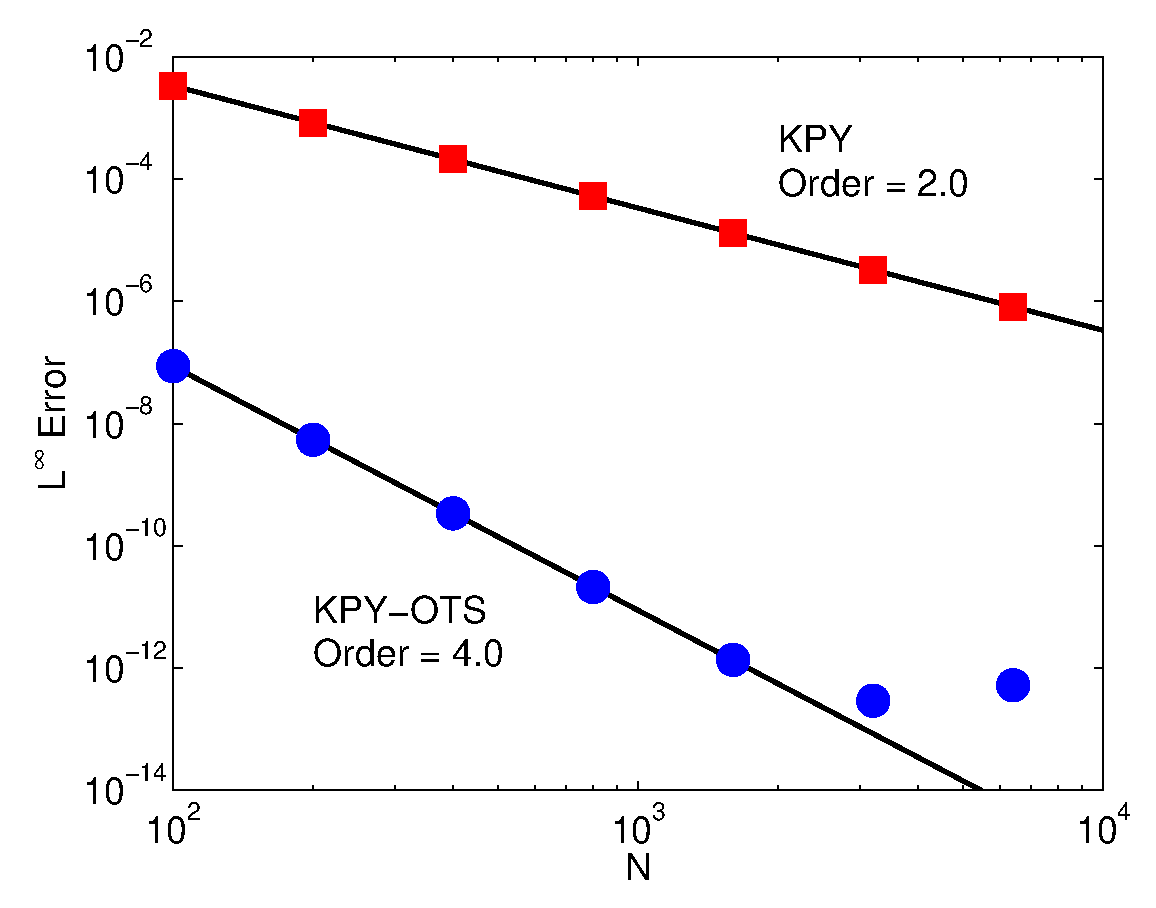
\includegraphics{figures/wave_eqn_1d_src_error_vs_N}}
\caption{$L^\infty$ error as a function of number of grid points for the
KPY discretization of the second-order wave equation on with OTS selection 
(blue circles) and without OTS selection (red squares).
}
\label{fig:wave_eqn_1d_error}
\end{center}
\end{figure}

\paragraph{High Accuracy Required for First Time Step}
For the KPY discretization of the wave equation, it is critical that a 
high-order accurate method is used to perform the first time step because 
the error introduced during this step affects the global error at all times.
Specifically, for the error of the KPY scheme to be $O(\dx^p)$, the numerical
solution at the first time step must be accurate to $O(\dx^{p+1})$.  In other 
words, the error introduced by the first time step must be at least one order
of accuracy higher than desired for the overall solution.

We can understand this need for higher-order accuracy of the first time step 
by solving the difference equation
\bea
  \frac{\he^{n+1} - 2 \he^{n} + \he^{n-1}}
       {\dt^2} = \dt^2 \lambda \he^{n}
  \label{eq:error_eqn_normal_mode},
\eea
for the normal modes of the error, 
where $\he$ is the coefficient of an arbitrary normal mode of the spatial
operator for the error $e \equiv u - \tu$.  The solution of this equation 
is~\cite{carrier_pearson_book}
\bea
  \he^n = \he^1 \frac{\kappa_+^n - \kappa_-^n}{\kappa_+ - \kappa_-} 
      + \he^0 \kappa_+ \kappa_- 
        \frac{\kappa_+^{n-1} - \kappa_-^{n-1}}{\kappa_+ - \kappa_-},
  \label{eq:error_eqn_normal_mode_soln}
\eea
where $\kappa_\pm$, the roots of the characteristic equation for 
(\ref{eq:error_eqn_normal_mode}), are given by~\cite{kreiss2002}
\beq
  \kappa_\pm = 1 + \frac{1}{2} \lambda \dt^2 
             \pm \dt \sqrt{\lambda + \frac{\lambda^2 \dt^2}{4}}.
\eeq
Notice that the denominator of both terms in 
(\ref{eq:error_eqn_normal_mode_soln}) is $O(\dt)$.  As a result, the 
global error is always at least one temporal order of accuracy less than the 
error in the initial conditions.  Therefore, the initial errors $e^0$ and 
$e^1$ must be $O(\dt^{p+1})$ in order to for the solution to be $O(\dt^p)$. 
For KPY without OTS selection, this observation indicates that the first
time step should be at least third-order accurate, which is exactly the way
that Kreiss \etal chose to compute the first time step in~\cite{kreiss2002}.
Because the OTS selection transforms KPY into a fourth-order accurate scheme, 
we require that the first time step is at least fifth-order accurate.

It is straightforward to construct a fifth-order approximation for the first 
time step by using a fifth-order Taylor series expansion in time:
\bea
  u^1 &=& u^0 + \dt u_t^0 + \frac{\dt^2}{2} u_{tt}^0
      + \frac{\dt^3}{6} u_{ttt}^0 
   + \frac{\dt^4}{24} u_{tttt}^0
  \nonumber \\
  &=& u^0 + \dt u_t^0 + \frac{\dt^2}{2} \left(c^2 u_{xx}^0 + f\right)
  \nonumber \\
  & & + \frac{\dt^3}{6} \left(c^2 \left(u_t\right)_{xx}^0 + f_t\right)
  \nonumber \\
  & & + \ \frac{\dt^4}{24} \left(c^4 u_{xxxx}^0 + c^2 f_{xx} + f_{tt}\right).
  \label{eq:KPY_fifth_order_first_step}
\eea
Note that sufficiently high-order accurate finite difference stencils may be 
used to compute some of the higher order terms in this expression.  However,
when advancing the solution using the optimal time step, special care must be 
exercised if finite differences are used to compute the derivatives in 
(\ref{eq:KPY_fifth_order_first_step}) because higher-order terms may be 
automatically (implicitly) included by lower-order terms in the expansion.


\subsubsection*{OTS Selection for Variable Coefficient Wave Equation}
We now consider the variable coefficient second-order wave equation
\beq
    u_{tt} - c(x)^2 u_{xx} = f,
    \label{eq:var_coef_wave_eqn}
\eeq
on the domain $0 < x < 1$.  Using the change of variables defined in 
(\ref{eq:change_of_variables}) and (\ref{eq:abar}), we can transform 
(\ref{eq:var_coef_wave_eqn}) into the constant-coefficient wave equation
\beq
  u_{tt} = \cbar^2 u_{yy} - \cbar c' u_y + f,
\eeq
where $c' = dc/dx$.


\paragraph*{OTS Selection on Transformed Domain}
On the transformed domain, it is straightforward to apply OTS selection 
because the leading-order spatial derivative has a constant coefficient.  
If we use second-order central differences for both the Laplacian and gradient 
terms (on a uniform grid in the transformed domain), the optimal time step is 
$\dt_{opt} = \dx/\cbar$ and the correction term, which is calculated by 
identifying the terms in $\left(\dt^2 \tu_{tttt}/12\right)$ that are not 
eliminated by the use of $\dt_{opt}$, is given by
\bea
  \frac{\dt^2}{12} 
  \left(
    \begin{array}{l}
        -2 \cbar^3 (c')_y u_{yy}
        -\cbar^3 (c')_{yy} u_{y}
        + \cbar^2 (c')^2 u_{yy} 
        \\
        +\ \cbar^2 c' (c')_y u_{y}
        + \cbar^2 f_{yy}
        - \cbar c' f_y
        + f_{tt}
    \end{array}
  \right).
\eea
Using the optimal time step and the correction term, we obtain a fourth-order
accurate KPY scheme for the variable coefficient wave equation 
(see Figure~\ref{fig:var_coef_wave_eqn_1d_error}).  As mentioned earlier,
a fifth-order accurate first time step is required to achieve this level of
accuracy.

\begin{figure}[thb]
\begin{center}
\scalebox{0.30}{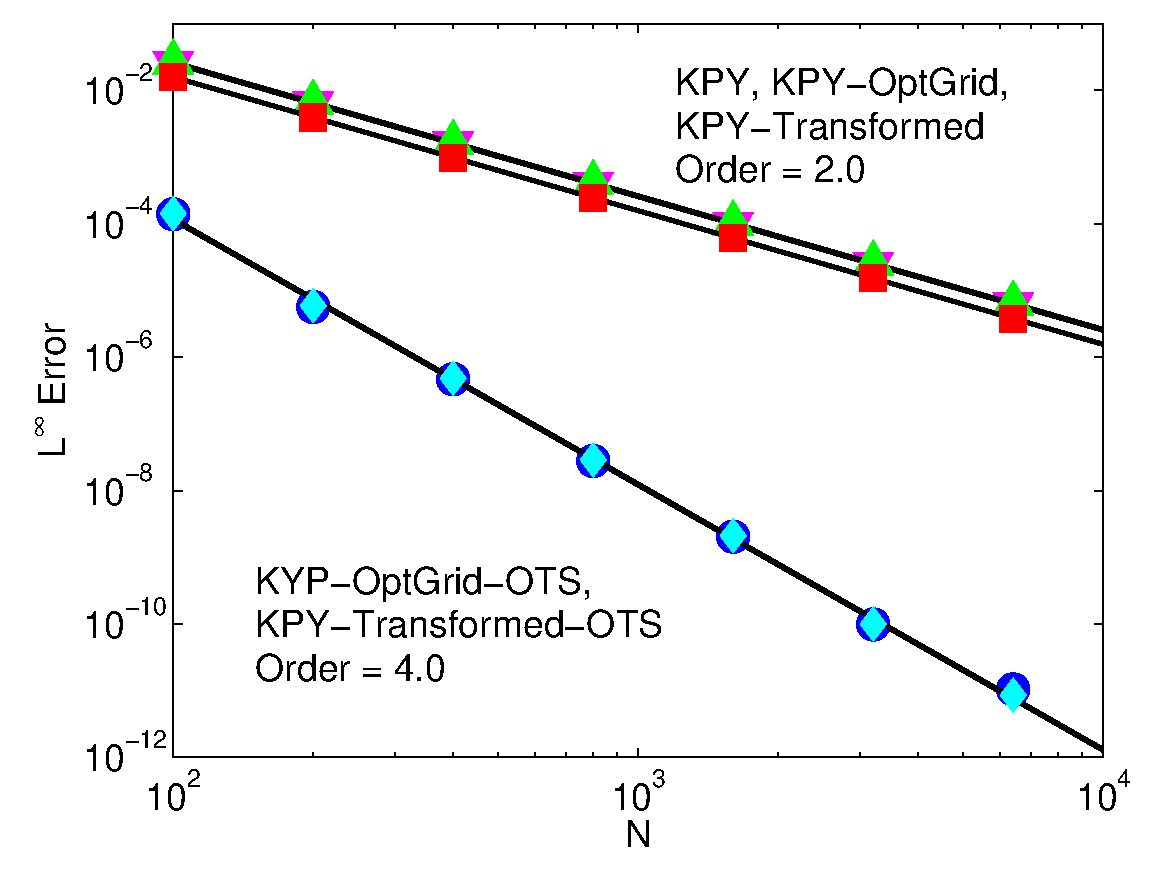
\includegraphics{figures/var_coef_wave_eqn_1d_error_vs_N}}
\caption{$L^\infty$ error as a function of number of grid points for various
KPY discretizations of the variable coefficient second-order wave equation:
KPY using a uniform grid on the original domain (red squares),
KPY using a uniform grid on the transformed domain (green triangles),
KPY using the optimal grid without OTS selection the original domain 
(magenta triangles),
KPY using a uniform grid with OTS selection on the transformed domain 
(cyan diamonds),
KPY using the optimal grid with OTS selection on the original domain 
(blue circles).  Note that the green triangles overlap the magenta triangles 
and the cyan diamonds overlap the blue circles. 
}
\label{fig:var_coef_wave_eqn_1d_error}
\end{center}
\end{figure}

\paragraph*{OTS Selection with Optimal Grid}
While applying OTS selection to the equation on the transformed domain yields the 
desired boost in order of accuracy, the lower-order spatial derivative and 
the correction term are tedious to deal with.  It is more convenient to 
work on the original domain but optimally choose the grid so that use of
an optimal time step still leads to fortuitous cancellation of the 
leading-order error.  

Following the procedure outlined in Section~\ref{sec:ots_var_coef_pdes}, we 
define the location of the grid points in the optimal grid by mapping
a uniform grid in the $y$-domain back to the $x$-domain and use 
the generalized finite difference approximation for the Laplacian 
(\ref{eq:laplacian_variable_grid}).  The optimal time step for the optimal
grid is given by $\dt_{opt} = \dy/\cbar$, where $\dy$ is the grid spacing 
in the $y$-domain.

The required correction term can be derived by first computing $u_{tttt}$ on 
the original domain
\bea
  u_{tttt} & = & 
    c^4 u_{xxxx} + 2 c^2 (c^2)_x u_{xxx} 
    + c^2 (c^2)_{xx} u_{xx} + \nonumber \\ 
& & c^2 f_{xx} + f_{tt}.
\eea
Using the heuristic mentioned in Section~\ref{sec:derivation_ots_corr_terms},
the terms involving $u_{xxxx}$ and $u_{xxx}$ are eliminated through the use 
of the optimal time step.  Thus, the correction term is
\beq
  \frac{\dt^2}{12} \left[ c^2 (c^2)_{xx} u_{xx} + c^2 f_{xx} + f_{tt} \right].
\eeq

As shown in Figure~\ref{fig:var_coef_wave_eqn_1d_error}, by using the optimal 
grid, optimal time step, and the correction terms, we are able to obtain a 
fourth-order accurate scheme for the variable coefficient wave equation on
the original domain.  The error on the variable-spaced grid is almost 
identical to the error obtained when solving the equation on the transformed 
domain. 


% DIFFUSION EQUATION FIGURE PLACED HERE TO SPREAD OUT FIGURES
\begin{figure}[thb]
\begin{center}
\scalebox{0.30}{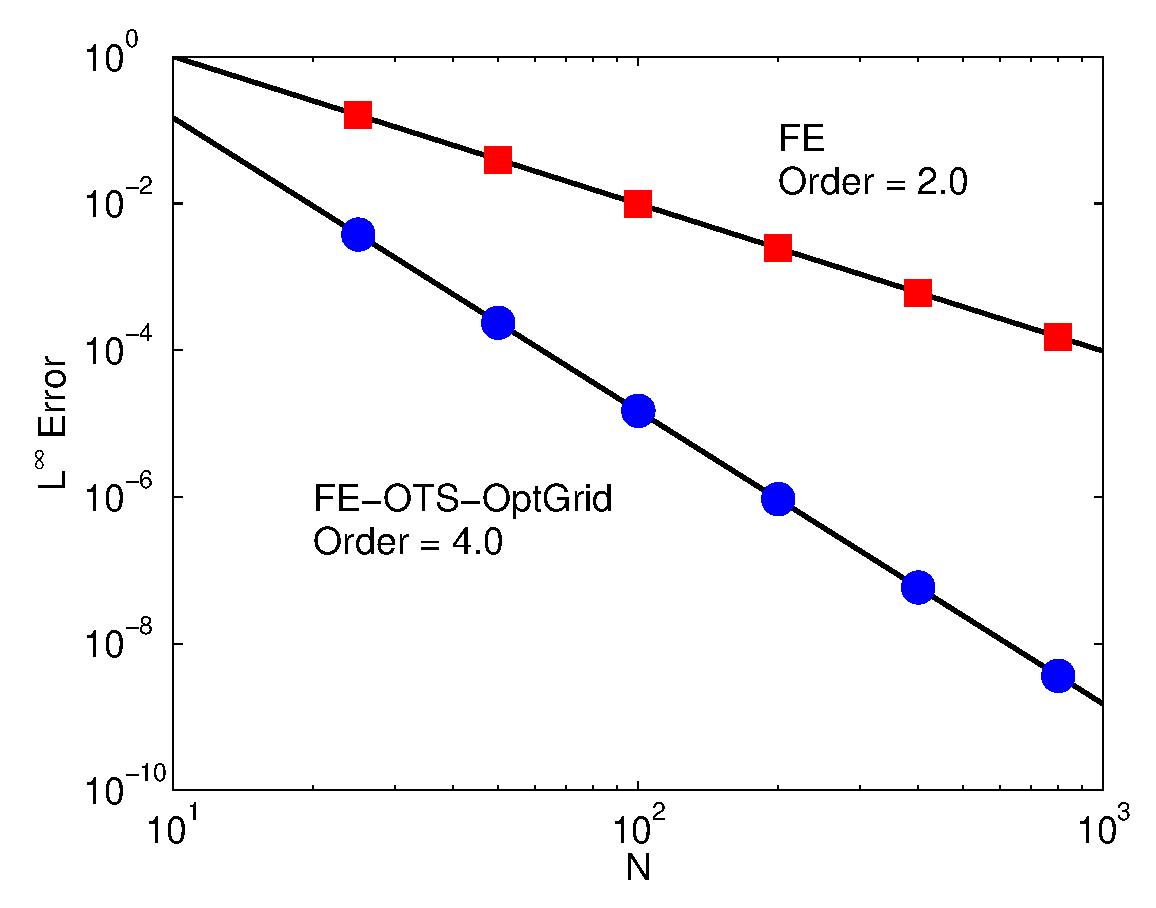
\includegraphics{figures/var_coef_diffusion_eqn_1d_error_vs_N}}
\caption{$L^\infty$ error as a function of number of grid points with 
OTS/Optimal Grid selection (blue circles) and on a uniform grid without 
OTS selection (red squares).
}
\label{fig:var_coef_diffusion_eqn_1d_error}
\end{center}
\end{figure}

\subsection{Application to Variable Coefficient Diffusion Equation}
In this section, we apply OTS and optimal grid selection to the 
variable-coefficient diffusion equation
\beq
  u_t = (D(x) u)_{xx} + f(x,t),
  \label{eq:var_coef_diffusion_eqn}
\eeq
on the domain $0 < x < 1$.  Note that we have expressed diffusion in a 
spatially inhomogeneous medium using the Fokker-Planck diffusivity 
law~\cite{vanmilligen2005}, which has been shown to often be more physically 
correct than Fick's law. 

Following the procedure outlined in Section~\ref{sec:ots_var_coef_pdes}, the
change of variables used to define the optimal grid is given by
$y = \dbar\int_0^x D(\xi)^{-1/2} d\xi$ where
$\dbar = \left(\int_0^1 D(\xi)^{-1/2} d\xi \right) ^ {-1}$.
Since the optimal time step for the constant coefficient diffusion equation 
is given by $\dto = \dx^2/6D$, the optimal time step for the variable
coefficient diffusion equation is given by $\dto = \left(\dy/\dbar\right)^2/6$.
The correction term for this scheme is 
\bea
  \frac{\dt^2}{2} \left[
  \begin{array}{c}
  6 D D_{xx} u_{xx} + 4 D D_{xxx} u_x D D_{xxxx} u + D f_{xx} \\
  + \ 6 D_x D_{xx} u_x + 2 D_x D_{xxx} u + 2 D_x f_x \\
  + \ D_{xx} u_t + f_t
  \end{array}
  \right]
\eea
which is derived by computing $u_{tt}$ and using the heuristic described in 
Section~\ref{sec:derivation_ots_corr_terms} to exclude the following terms:
\beq
  D^2u_{xxxx} \ , \ 4 D D_x u_{xxx} \ , \ 
  2 D_x D u_{xxx} \ , \ 6 \left(D_x\right)^2 u_{xx}.
\eeq
Combining the optimal grid, optimal time step, and the correction term, we are 
able to obtain fourth-order solutions for (\ref{eq:var_coef_diffusion_eqn})
using only a formally second-order FD scheme (see 
Figure~\ref{fig:var_coef_diffusion_eqn_1d_error}).  
Figure~\ref{fig:var_coef_diffusion_eqn_1d_solns} shows a comparison of 
solutions computed with and without the optimal grid and OTS selection.

\begin{figure}[tbh]
\begin{center}
\scalebox{0.24}{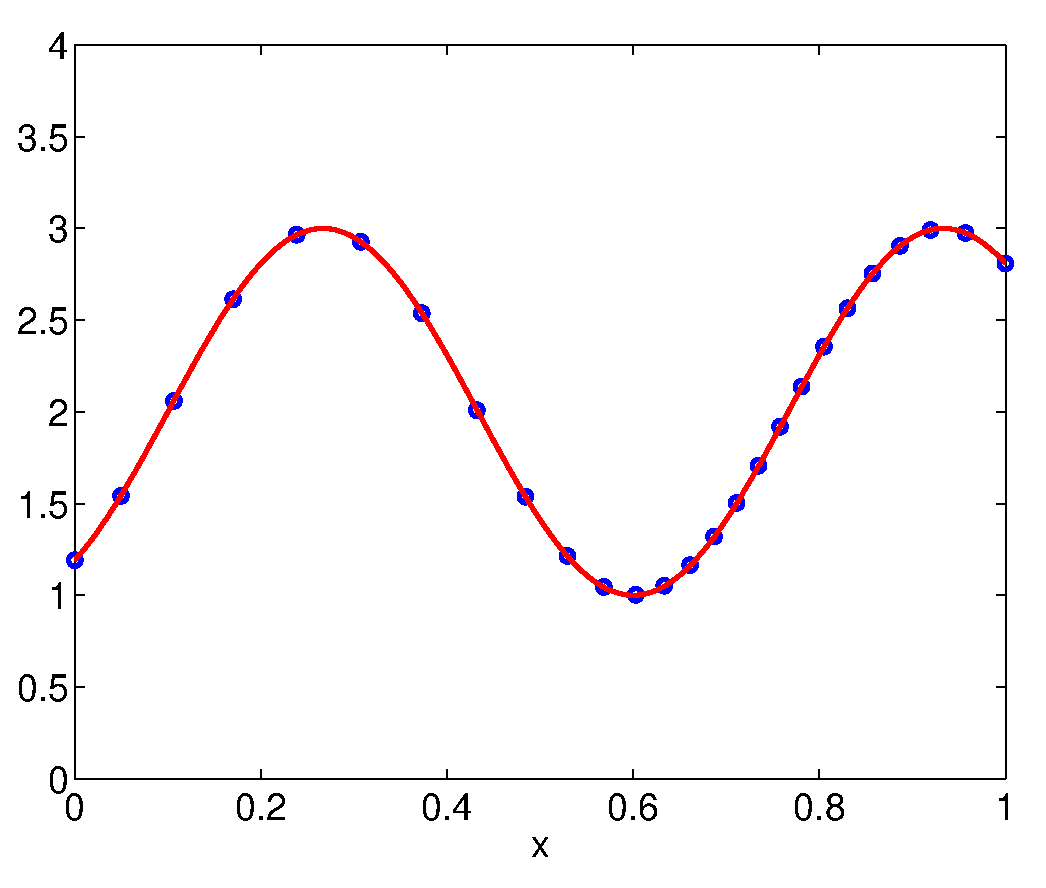
\includegraphics{figures/var_coef_diffusion_eqn_1d_FE_OTS_OptGrid_soln}} \ 
\scalebox{0.24}{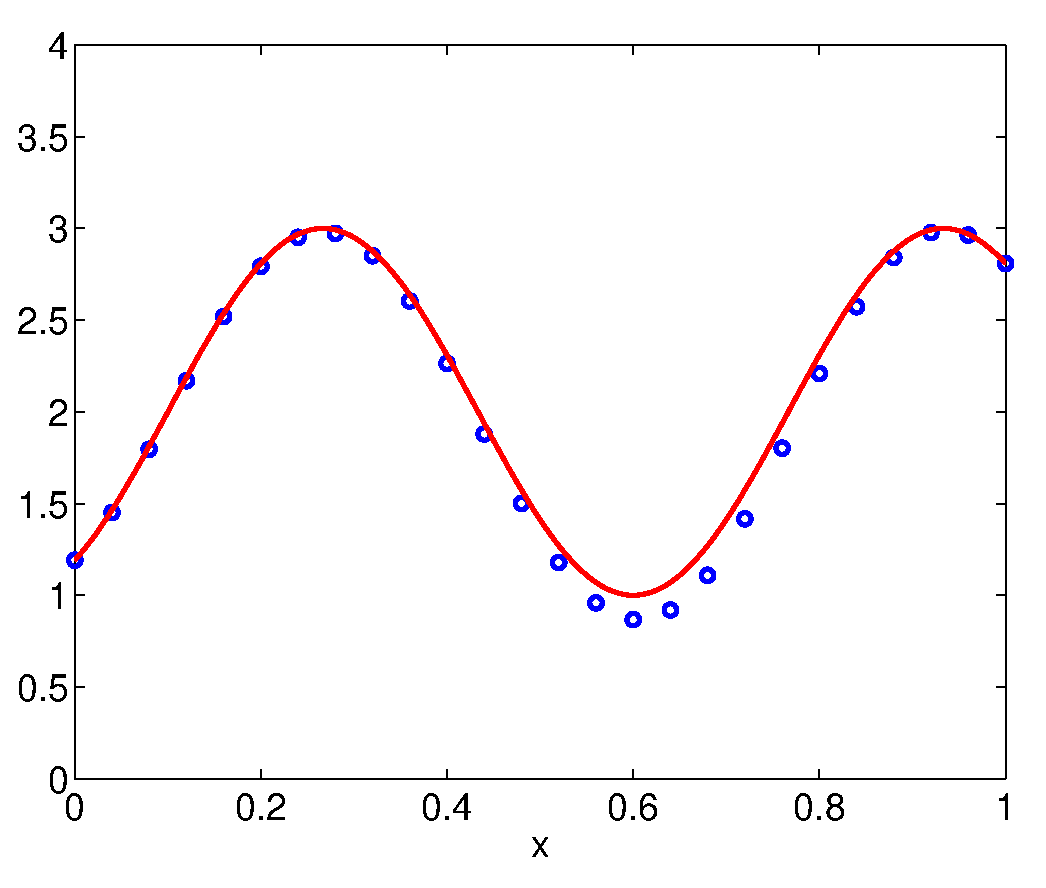
\includegraphics{figures/var_coef_diffusion_eqn_1d_FE_soln}}
\caption{Comparison of numerical solutions for the variable coefficient
diffusion equation~(\ref{eq:var_coef_diffusion_eqn}) computed using 
the optimal grid and OTS selection (left) and a uniform grid without OTS
selection (right).  Both figures compare the analytical solution (solid line)
with the numerical solution (circles) computed using $25$ grid points.
}
\label{fig:var_coef_diffusion_eqn_1d_solns}
\end{center}
\end{figure}


\section{Summary and Conclusions}
In this paper, we have extended the philosophy of optimizing the parameters
of FD schemes (\eg the time step size) for accuracy to the selection of the 
computational grid.  In particular, we have presented a method to boost the 
order of accuracy of FD schemes for PDEs where the leading-order spatial derivative has a 
variable coefficient by using an optimal time step and an optimal grid.  We have 
described the basic procedure for constructing the optimal grid, computing the optimal time step, 
and deriving the required correction terms.  To demonstrate the power of these 
techniques, we have applied them to the variable coefficient wave equation and 
the Fokker-Planck form of the diffusion equation in an inhomogeneous medium.  
Our analysis of the KPY scheme (used to solve the wave equation) also serves 
as an example of OTS selection applied to multistep time integration schemes.  


\subsection{Future Work}
An important direction for future work is the generalization of the current 
work to PDEs in higher spatial dimensions.  We believe that the use of a 
change of variables may still be viable.  However, we may need to allow for a change in the shape 
of domain and the possibility that the optimal grid may no longer be orthogonal.  
Both of these issues complicate the construction of the finite difference
scheme on the original domain. 


\bibliography{OTSPDE-WCE2009}

\end{document}


% >>>>>>>>>>>>>>>>>>>>>> Bibliography <<<<<<<<<<<<<<<<<<<<<<<<<<<<<<<<<<<<<
% A label is give for each bibitem.  Your paper references this label

%\begin{thebibliography}{99}
%
%% >>>>>>>>> Book examples <<<<<<<<<
%\bibitem{CarpenterBOOK} Carpenter, R.H.S., {\it Movements of the Eyes},
% 2nd Edition, Pion Publishing, 1988.
%
%\bibitem{FranklinBOOK} Franklin, G.F., Powel, J.D., Workman, M.L.,
%{\it Digital Control of Dynamic Systems}, Second Edition,
%Addison-Wesley, 1990.
%
%% >>>>>>>>> Conference Proceedings Example <<<<<<<<<
%\bibitem{OhICRA1998} Oh, P.Y., Allen, P.K., ``Design a Partitioned
% Visual Feedback Controller,'' {\it IEEE Int Conf Robotics
% \& Automation}, Leuven, Belgium, pp. 1360-1365 5/98
%
%% >>>>>>>>> Journal Example <<<<<<<<<<<<<<<<<<<<<<<<
%\bibitem{OhTRA2001} Oh, P.Y., Allen, P.K., ``Visual Servoing
% by Partitioning Degrees of Freedom,'' {\it IEEE Trans on
% Robotics \& Automation}, V17, N1, pp. 1-17, 2/01
%
%\end{thebibliography}
\end{document}
